\documentclass{beamer}[10]


%
% macro
%

\usepackage{pgf}
\usepackage[english]{babel}
\usepackage[utf8]{inputenc} % use unicode chars
\usepackage{lmodern}% http://ctan.org/pkg/lm
\usepackage{beamerthemesplit}
\usepackage{graphics,epsfig,subfigure}
\usepackage{url}
\usepackage{srcltx}
\usepackage{hyperref}
\usepackage[mathescape,escapeinside=||]{minted}
\usepackage{import}
\usepackage{mathtools}
\usepackage{amsmath}
\usepackage{color}
%\usepackage[beamer]{hf-tikz}
\usepackage{xfrac}
\usepackage{makeidx}
\usepackage{multicol}

%\showboxdepth=5
%\showboxbreadth=5

% Slides in 16:9
\usepackage[orientation=landscape,size=custom,width=16,height=9,scale=0.5,debug]{beamerposter} 

%
% Macros
%
\definecolor{darkred}{rgb}{0.55, 0.0, 0.0}
\definecolor{light-gray}{gray}{.80}
\definecolor{light-yellow}{rgb}{255,255,153}
\definecolor{alizarin}{rgb}{0.82, 0.1, 0.26}
% colorized font
\newcommand{\red}[1] {{\color{red} #1}}
\newcommand{\darkred}[1] {{\color{darkred} #1}}
\newcommand{\blue}[1] {{\color{blue} #1}}
\newcommand{\green}[1] {{\color{green} #1}}
\newcommand{\gray}[1] {{\color{gray} #1}}
\newcommand{\grey}[1] {{\color{gray} #1}}

\newcommand{\hearts} {\red{$\heartsuit$}}
\newcommand{\diamonds} {\red{$\diamondsuit$}}
\newcommand{\spades} {$\spadesuit$}
\newcommand{\clubs} {$\clubsuit$}
\newcommand{\pyoptional}[1]{\diamonds #1 \diamonds}

\newcommand{\deltasum}[1]{\sum (#1 - \bar{#1})}
\newcommand{\deltasumsq}[1]{\sum (#1 - \bar{#1})^{2}}

%
% Take care of the newline after \frametitle
%
\newenvironment{pyframe}[1]
{\begin{frame}[fragile,environment=pyframe]\frametitle{#1}
 
}
{\end{frame}}


% environments
\newminted{py}{mathescape,escapeinside=||}% 
\newminted{bash}{mathescape,escapeinside=||}%

% python highlights: module, method
\newcommand{\pymodule}[1]{\darkred{\textbf{#1}}}
\newcommand{\pyfunction}[1]{\textit{#1}}
\newcommand{\keyword}[1]{\texttt{#1}}
\newcommand{\pyver}[1]{\colorbox{yellow}{#1}}
\newcommand{\typeonly}[1]{\colorbox{green}{#1}}
\newcommand{\pyvers}[1]{\raisebox{0em}{\colorbox{yellow}{#1}}}
\newcommand{\code}[1] { \texttt{#1} }

% special symbils
\newcommand{\mymapsto}{\operatornamewithlimits{\longmapsto}}

\makeatletter
\newcommand{\xMapsto}[2][]{\ext@arrow 0599{\Mapstofill@}{#1}{#2}}
\def\Mapstofill@{\arrowfill@{\Mapstochar\Relbar}\Relbar\Rightarrow}
\makeatother




%
% style
%

\setbeamercovered{transparent}
\mode<presentation>

%\geometry{top=5pt, margin=5pt}
%The outertheme defines the head and the footline of each slide
% \setbeamercolor{block title}{bg=orange}
% \useinnertheme{circles}
% \useoutertheme{split}
%\beamertemplatenavigationsymbolsempty

%\usetheme[numbers,totalnumber,compress,sidebarshades]{Babel}
\setbeamertemplate{headline}{
 \leavevmode%
  \hbox{%
%,bb=0 0 5cm 2cm
    \hspace{5pt}\includegraphics[height=1.2cm]{logo.eps}
    \hspace{240pt}\includegraphics[height=1.2cm]{logo.eps}
    }
}
\setbeamertemplate{footline}{
\noindent\textbf{\hspace{5pt}\insertsection \insertsubsection\hfill}\textbf{\hfill{\color{gray}\insertshortauthor}\hfill}\textbf{\hfill }
   % \textline[t]{ \insertsection  \insertsubsection}{\gray{\insertshortauthor}}{right}
}
%\useinnertheme[shadow=false]{rounded}
% frametitle
\setbeamertemplate{frametitle}[default][center]
\setbeamercolor*{frametitle}{bg=white,fg=gray,parent=palette primary}
\setbeamerfont{frametitle}{series=\bfseries,size={\fontsize{16}{8}}}
% table of contents
\setbeamercolor{section in toc}{fg=black} % series=\bfseries,size={\fontsize{16}{8}}}
%\setbeamercolor{section/subsection in toc}{fg=black}
%\setbeamercolor{subsection in toc}{fg=black}
%\setbeamerfont{section in toc}{fg=black} % series=\bfseries,size={\fontsize{16}{8}}}
%\setbeamerfont{section/subsection in toc}{fg=black}
%\setbeamerfont{subsection in toc}{fg=black}

%title
\setbeamercolor{title}{fg=black,bg=white}
\setbeamerfont{title}{series=\bfseries,size={\fontsize{24.88}{32}}}
%subtitle
\setbeamercolor{subtitle}{fg=gray}
\setbeamerfont{subtitle}{series=\bfseries,size={\fontsize{14}{}}}
%titlepage
\setbeamertemplate{title page}[default][center]
% bullets
\setbeamercolor{itemize item}{fg=gray}
\setbeamertemplate{itemize items}[circle]
\setbeamercolor{itemize item}{fg=light-gray}
\setbeamercolor{itemize items}{fg=light-gray}
% enumerations
\setbeamercolor{enumerate item}{fg=black}
\setbeamercolor{local structure}{fg=black}

%
% increase itemize spacing
%
%\newlength{\wideitemsep}
%\setlength{\wideitemsep}{\itemsep}
%\addtolength{\wideitemsep}{14pt}
%\let\olditem\item
%\renewcommand{\item}{\setlength{\itemsep}{\wideitemsep}\olditem}

  % \usecolortheme[named=orange]{structure}
  % \useinnertheme{circles}
  % \usefonttheme[onlymath]{serif}
\setbeamercovered{transparent}
  % \setbeamertemplate{blocks}[rounded][shadow=true]

\makeindex


\title{Scaling MySQL with Python}
\subtitle{EuroPython 2015, $22^{th}$ July - Bilbao}
\author{Roberto Polli - \href{mailto:roberto.polli@par-tec.it}{roberto.polli@par-tec.it}}
\date{21-27 July 2015}
\institute{Par-Tec Spa - Rome Operation Unit\\
    P.zza S. Benedetto da Norcia, 33\\
    00040, Pomezia (RM) - www.par-tec.it}

%
%
\begin{document}

%% cover
\frame{\titlepage 
\vspace{-0.5cm}
}

%% agenda
\iffalse
\frame{\frametitle{Agenda}
\tiny
\tableofcontents%[pausesection]
}
\fi

%% Starting doc
\section{Intro}
\frame{ \frametitle{Who? What? Why?}
\begin{itemize}

\item Manage, replicate, scale MySQL databases with python
\\

\item Roberto Polli - Solutions Architect @ par-tec.it. Loves writing in C,
Java and Python. Red Hat Certified Engineer and Virtualization
Administrator.
\\
\\
\item Par-Tec – Proud sponsor of this talk ;) Contributes to various FLOSS. \\
Provides expertise in IT Infrastructure \& Services and \\ Business Intelligence
solutions + Vertical Applications for the financial market.

\end{itemize}
}

\begin{pyframe}{Agenda}
\begin{itemize}
\item MySQL architecture
\item Getting informations
\item Comparing databases
\item Replication 2.0 aka GTID
\item Fabric: scaling & sharding for the masses
%\item modules: \pymodule{scipy, matplotlib}
\end{itemize}
\end{pyframe}


\begin{pyframe}{MySQL Architecture}
\begin{itemize}
\item MySQL is not only SQL
% Query parser vs engine store
\item Architecture of a database
% query parser, cache, transaction log, MVCC
% http://www.oracle.com/technetwork/articles/javase/figure2-large-145676.jpg
\item MVCC
\item Replication
\item Consistency is here to stay
%
\end{itemize}
\end{pyframe}


\begin{pyframe}{MySQL Architecture}
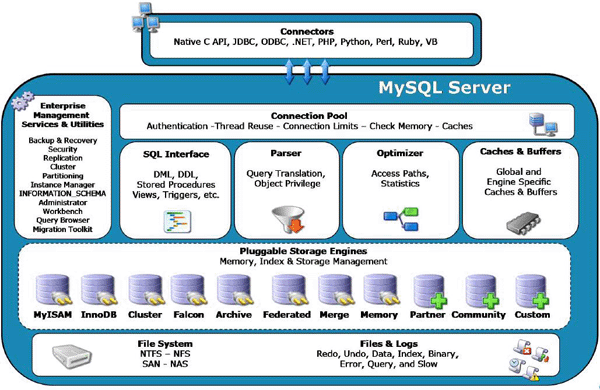
\includegraphics[height=5.5cm]{mysql-architecture.pdf}
{\large
\begin{center}
It's a lot of stuff
\end{center}
}
\end{pyframe}


\begin{pyframe}{MySQL Architecture}
% Map in the figure every task
We should manage and monitor
\begin{itemize}
\item Database size: Tables, Indexes, Binary Logs
\item Replication inconsistencies
\item Failover
\end{itemize}
Can all of this be simpler?
\end{pyframe}


\begin{pyframe}{Make it simple}
Yes!
\begin{minted}{bash}
# wget https://dev.mysql.com/get/Downloads/MySQLGUITools/mysql-utilities-1.6.1.tar.gz
# tar xf mysql-utilities-1.6.1.tar.gz
# python setup.py install
\end{minted}{bash}
or
\begin{minted}{bash}
# yum -y install https://dev.mysql.com/get/mysql-community-release-el7-5.noarch.rpm
# yum -y install mysql-utilites
\end{minted}{bash}
\end{pyframe}


\begin{pyframe}{Preparing your setup}
Avoid typing credentials!
\begin{minted}{bash}
# cat /etc/my.cnf
# This is the client stanza of my.cnf
[mysql]
user=fabric
password=fabric
\end{minted}{bash}
and
\begin{minted}{bash}

\end{minted}{bash}
\end{pyframe}




\begin{pyframe}{Single Entrypoint: mysqluc}
Start with \code{mysqluc}

\begin{itemize}
\item An entrypoint for all utilities
\item Contextual help
\item TAB completion
\end{itemize}
\end{pyframe}


\iffalse
\begin{pyframe}{Managing binlog}
Managing binlog with \code{mysqlbinlogmove} and
\code{mysqlbinlogpurge}
\end{pyframe}
\fi


\begin{pyframe}{Disk usage}
A single command to show all disk usage infos (excluded system logs)

\begin{minted}{bash}
$ mysqldiskusage --server=root:secret@s-1.docker --all |grep -- =
Total database disk usage = 7601892 bytes or 7.25 MB
Current binary log file = s-1-bin.000009
Total size of binary logs = 231 bytes
\end{minted}{bash}

\end{pyframe}

%
% Exporting and Importing
%
\begin{pyframe}{Export - I}
You can forget mysqldump and use the following
command for complete and consistent backup.
\begin{minted}{bash}
$ mysqldbexport > data.sql \
--server=root:root@localhost:13001
--all
\end{minted}{bash}
% --export=master --rpl=master --rpl-user=rpl:rpl

Attention: to backup big databases, use InnoDB engine
and an InnoDB backup tool!
\end{pyframe}


\begin{pyframe}{Import - I}
Then import the dump with
\begin{minted}{bash}
$mysqldiff \
    --server1=root:root@master:3306 \
    --server2=root:root@slave:3306 \
    sakila:sakila --changes-for=server2
\end{minted}
To provision a new slave we'll use a similar
procedure with some variants.
\end{pyframe}






%
% Comparing
%
\begin{pyframe}{Comparing databases - I}
To compare databases, use
\begin{minted}{bash}
#mysqldbcompare \
    --server1=root:root@master:3306 \
    --server2=root:root@slave:3306 \
    sakila -a --difftype=SQL \
    --show-reverse --quiet
\end{minted}{bash}
\end{pyframe}


\begin{pyframe}{Comparing databases - II}
We can create the statemets to fix the differences!
\begin{minted}{bash}
#mysqldiff \
    --server1=root:root@master:3306 \
    --server2=root:root@slave:3306 \
    sakila:sakila --changes-for=server2
\end{minted}{bash}
\end{pyframe}


%
% replication
%
\begin{pyframe}{Replication 2.0}
MySQL 5.6+ replication is based on Global Transaction ID
\begin{itemize}
\item Every server has a unique UUID \\
\code{3E11FA47-71CA-11E1-9E33-C80AA9429562}

\item This makes every TransactionID a Global one
\code{3E11FA47-71CA-11E1-9E33-C80AA9429562:32}
\end{itemize}
GTIDs avoid loops in replication!
\end{pyframe}


\begin{pyframe}{Configuring replication}
\begin{itemize}
\item In MySQL replication is configured on the slave only.
\item The slave connects to the master with a provisioned
 user and gets its changelog (binlog).
\end{itemize}
%% IMAGE
If binlog had been purged, you need to import the
master database first!
\end{pyframe}


\begin{pyframe}{Configuring replication}
mysqlreplicate takes care of
\begin{itemize}
\item provisioning the replica user on the master;
\item get a suitable GTID;
\item configure the slave to point to the master.
\end{itemize}
\begin{minted}
mysqlreplicate \
 --master=root:pass@master \
 --slave=root:pass@slave \
 --rpl-user=repl:rpass \
 -b

# master on 192.168.1.1: ... connected.
# slave on 192.168.1.2: ... connected.
# Checking for binary logging on master...
# Setting up replication...
# ...done.
\end{minted}
Obviously
\end{pyframe}

\begin{pyframe}{Configuring replication -II}
You can provision a new slave creating a suitable dump
with mysqldbexport. Just:
\begin{itemize}
\item check that replica user is provisioned on the master;
\item create a custom dump.sql;
\item add --export=master;
\end{itemize}
\begin{minted}
cat > data.sql <<EOF
-- ignore previous changelogs
-- and trust the backup only
STOP SLAVE;
RESET MASTER;
COMMIT;

EOF

mysqldbexport >> data.sql \
 --server=root:pass@master \
 --rpl-user=repl:rpass \
 --export=master \
 --rpl=master \
 --all

mysqldbimport --server=root:root@slave \
 data.sql
\end{minted}
\end{pyframe}



\begin{pyframe}{Failover - I}
mysqlfailover, requires report-host
\end{pyframe}


\begin{pyframe}{Failover - II}
example failover
\end{pyframe}

\begin{pyframe}{Fabric - I}
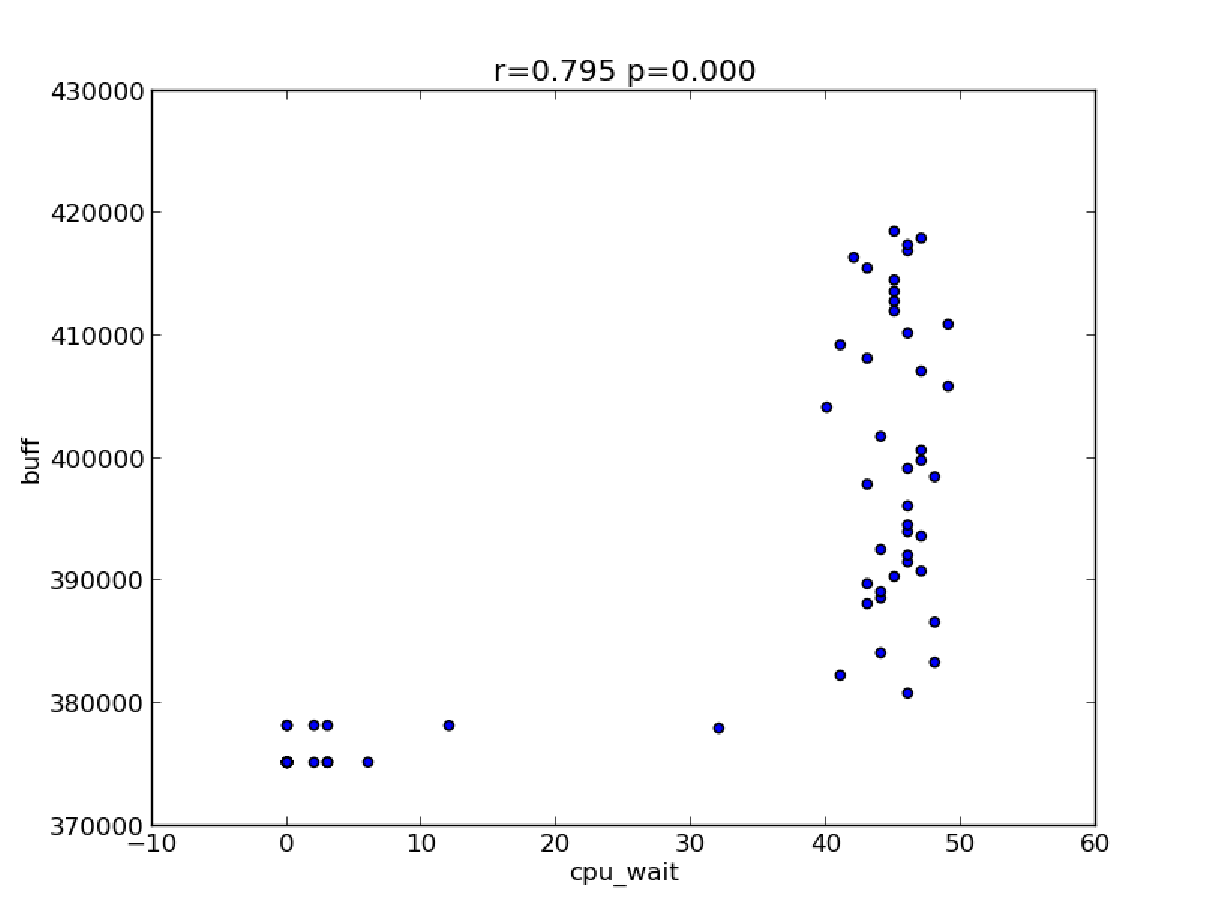
\includegraphics[height=6.6cm,width=12cm]{monochromo_cpu_wait_buff.pdf}
\end{pyframe}

\begin{pyframe}{Fabric - II}
\end{pyframe}


\begin{pyframe}{Wrap Up}
\begin{itemize}
\item Use MySQL Utilities
\item Enjoy replicatioon
\item Don't reingest failed master
\item Try Fabric
\end{itemize}
\end{pyframe}


\iffalse
\begin{pyframe}{mysqlbackup \-\-what}
To make a consistent backup you need to know
 how your data are stored (engine, ...).
 Are you sure your backup is:
\begin{itemize}
\item consistent?
\item usable?
\item without side effect?
\end{itemize}
Curious? Attend `MySQL for Pythonistas' on FIXME
\end{pyframe}
\fi


\begin{pyframe}{That's all folks!}
\begin{center}
Thank you for the attention! \\\\
\insertauthor
\end{center}
\end{pyframe}


\end{document}
